\documentclass[border=6pt]{standalone}
\usepackage{tikz}
\usepackage{pgfplots}
\pgfplotsset{compat=1.18}
\usetikzlibrary{arrows.meta,positioning,shapes.geometric,fit,backgrounds,calc,decorations.pathreplacing,patterns,pgfplots.groupplots}
\tikzset{
  blk/.style={rectangle, rounded corners=2pt, draw=black!70, thick, fill=blue!6,
              minimum height=8mm, minimum width=20mm, align=center, font=\small},
  io/.style={rectangle, rounded corners=6pt, draw=black!70, thick, fill=green!8,
             minimum height=8mm, align=center, font=\small},
  proc/.style={rectangle, draw=black!70, thick, fill=orange!10, minimum height=8mm,
               align=center, font=\small},
  dec/.style={diamond, aspect=2, draw=black!70, thick, fill=yellow!15, align=center, font=\footnotesize},
  warnbox/.style={rectangle, rounded corners=2pt, draw=red!60!black, thick, fill=red!7,
                  minimum height=8mm, align=center, font=\small},
  oklbox/.style={rectangle, rounded corners=2pt, draw=green!45!black, thick, fill=green!8,
                 minimum height=8mm, align=center, font=\small},
  ar/.style={-{Latex[length=2mm]}, thick},
  arl/.style={-{Latex[length=2mm]}, thick, dashed, draw=black!55},
  lbl/.style={font=\footnotesize\itshape, text=black!60},
}
\definecolor{good}{RGB}{34,139,34}
\definecolor{bad}{RGB}{178,34,34}
\definecolor{warn}{RGB}{218,165,32}
\definecolor{pesblue}{RGB}{0,45,98}
\definecolor{complete}{RGB}{30,125,79}
\definecolor{partial}{RGB}{176,106,0}
\definecolor{blocked}{RGB}{166,43,43}
% --- figure-local styles -------------------------------------------------
\tikzset{
  stage/.style={text width=19mm, minimum height=14mm, inner sep=2pt},
  minibox/.style={text width=19mm, minimum height=12mm, inner sep=2pt, font=\scriptsize},
  linklbl/.style={font=\scriptsize\itshape, text=black!60, align=center, text width=22mm},
  notrun/.style={rectangle, rounded corners=2pt, draw=black!35, dashed, fill=black!4,
                 text=black!55, align=center, font=\scriptsize,
                 text width=19mm, minimum height=12mm, inner sep=2pt},
}
\begin{document}
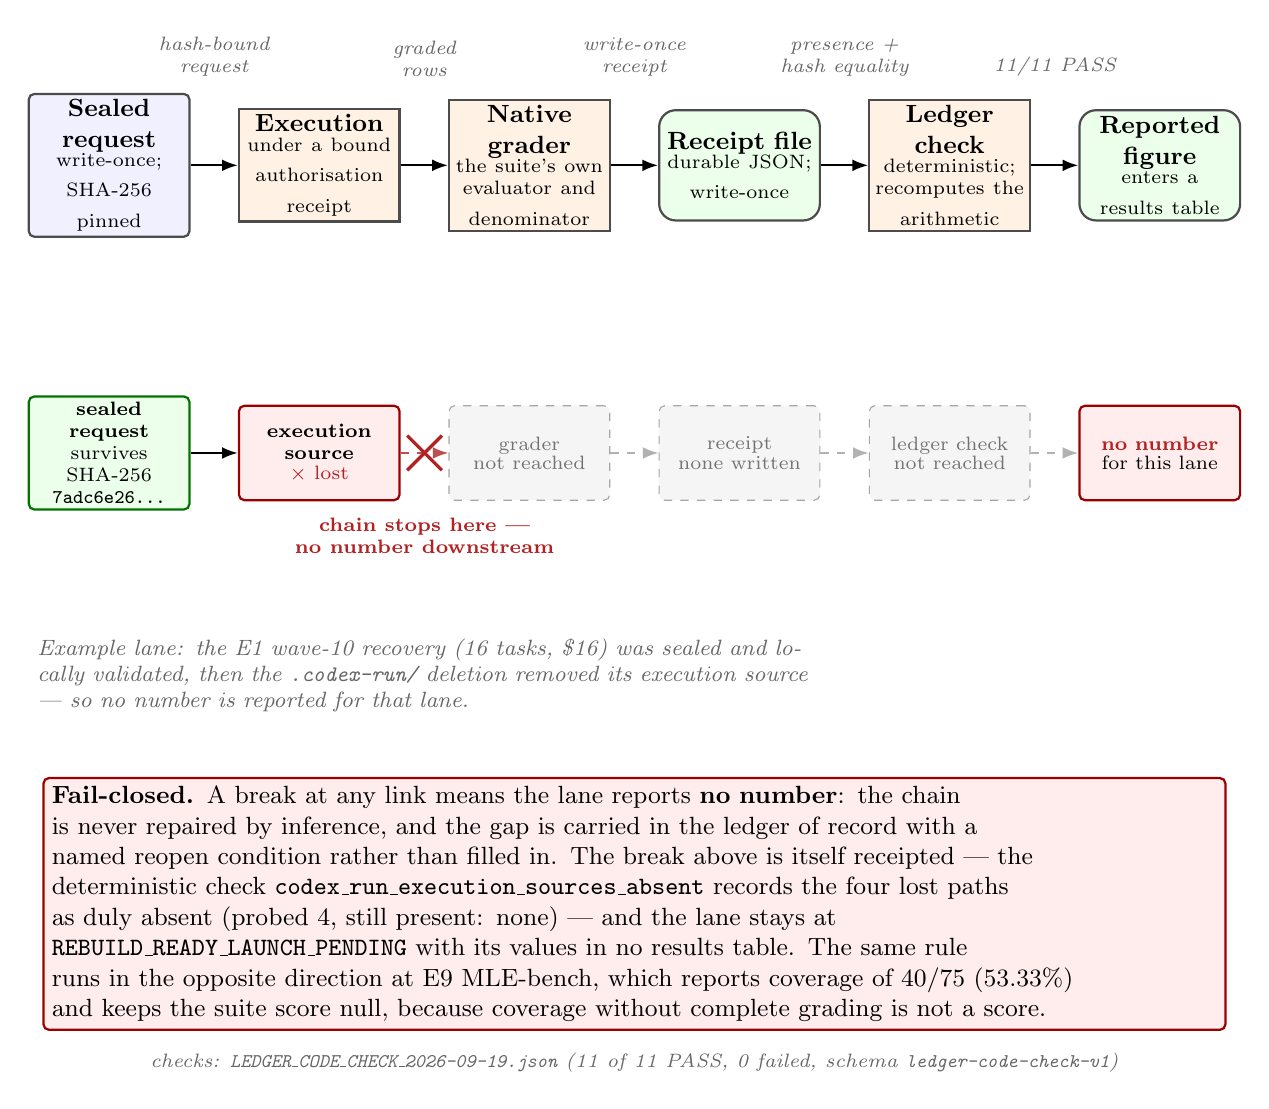
\begin{tikzpicture}

  % ============ the chain: one sealed request to one reported number ============
  \node[blk, stage] (s1)
    {\textbf{Sealed request}\\[-1pt]{\scriptsize write-once;\\ SHA-256 pinned}};
  \node[proc, stage, right=6mm of s1] (s2)
    {\textbf{Execution}\\[-1pt]{\scriptsize under a bound\\ authorisation receipt}};
  \node[proc, stage, right=6mm of s2] (s3)
    {\textbf{Native grader}\\[-1pt]{\scriptsize the suite's own\\ evaluator and\\ denominator}};
  \node[io, stage, right=6mm of s3] (s4)
    {\textbf{Receipt file}\\[-1pt]{\scriptsize durable JSON;\\ write-once}};
  \node[proc, stage, right=6mm of s4] (s5)
    {\textbf{Ledger\\ check}\\[-1pt]{\scriptsize deterministic;\\ recomputes the\\ arithmetic}};  \node[io, stage, right=6mm of s5] (s6)
    {\textbf{Reported figure}\\[-1pt]{\scriptsize enters a\\ results table}};

  \draw[ar] (s1) -- (s2)
    node[lbl, linklbl, midway, above=10mm] {hash-bound\\ request};
  \draw[ar] (s2) -- (s3)
    node[lbl, linklbl, midway, above=10mm] {graded\\ rows};
  \draw[ar] (s3) -- (s4)
    node[lbl, linklbl, midway, above=10mm] {write-once\\ receipt};
  \draw[ar] (s4) -- (s5)
    node[lbl, linklbl, midway, above=10mm] {presence +\\ hash equality};
  \draw[ar] (s5) -- (s6)
    node[lbl, linklbl, midway, above=10mm] {11/11 PASS};

  % ============ one broken link: E1 wave-10 ============
  \node[oklbox, minibox, below=20mm of s1] (b1)
    {\textbf{sealed request}\\ survives\\ {\scriptsize SHA-256\\ \texttt{7adc6e26\ldots}}};
  \node[warnbox, minibox] (b2) at (b1 -| s2)
    {\textbf{execution\\ source}\\[-1pt]{\scriptsize\textcolor{bad}{$\times$ lost}}};
  \node[notrun] (b3) at (b1 -| s3)
    {grader\\[-1pt]{\scriptsize not reached}};
  \node[notrun] (b4) at (b1 -| s4)
    {receipt\\[-1pt]{\scriptsize none written}};
  \node[notrun] (b5) at (b1 -| s5)
    {ledger check\\[-1pt]{\scriptsize not reached}};
  \node[warnbox, minibox] (b6) at (b1 -| s6)
    {\textbf{\textcolor{bad}{no number}}\\[-1pt]{\scriptsize for this lane}};

  \draw[ar] (b1) -- (b2);
  \draw[arl, draw=bad!80] (b2) -- (b3);
  \draw[arl, draw=black!30] (b3) -- (b4);
  \draw[arl, draw=black!30] (b4) -- (b5);
  \draw[arl, draw=black!30] (b5) -- (b6);

  % the break itself
  \coordinate (brk) at ($(b2.east)!0.5!(b3.west)$);
  \draw[bad, very thick] ($(brk)+(-2.2mm,2.2mm)$) -- ($(brk)+(2.2mm,-2.2mm)$);
  \draw[bad, very thick] ($(brk)+(-2.2mm,-2.2mm)$) -- ($(brk)+(2.2mm,2.2mm)$);
  \node[font=\scriptsize\bfseries, text=bad, anchor=north, align=center]
    at ($(brk)+(0,-7mm)$) {chain stops here ---\\ no number downstream};

  % what the break was
  \node[lbl, anchor=north west, align=left, text width=100mm] (cause)
    at ($(b1.south west)+(0,-15mm)$)
    {Example lane: the E1 wave-10 recovery (16 tasks, \$16) was sealed and
     locally validated, then the \texttt{.codex-run/} deletion removed its
     execution source --- so no number is reported for that lane.};
  \coordinate (cx) at ($(b1.west)!0.5!(b6.east)$);
  \coordinate (fcN) at (cause.south -| cx);

  % ============ fail-closed rule ============
  \node[warnbox, anchor=north, align=left, text width=148mm, inner sep=3pt] (fc)
    at ($(fcN)+(0,-7mm)$)
    {\raggedright\textbf{Fail-closed.} A break at any link means the lane reports
     \textbf{no number}: the chain\\
     is never repaired by inference, and the gap is carried in the ledger of
     record with a\\
     named reopen condition rather than filled in. The break above is itself
     receipted --- the\\
     deterministic check \texttt{codex\_run\_execution\_sources\_absent}
     records the four lost paths\\
     as duly absent (probed 4, still present: none) --- and the lane stays at\\
     \texttt{REBUILD\_READY\_LAUNCH\_PENDING} with its values in no results
     table. The same rule\\
     runs in the opposite direction at E9 MLE-bench, which reports coverage of
     40/75 (53.33\%)\\
     and keeps the suite score null, because coverage without complete grading
     is not a score.};

  \node[lbl, anchor=north, align=center]
    at ($(fc.south)+(0,-1.5mm)$)
    {\scriptsize checks: \texttt{LEDGER\_CODE\_CHECK\_2026-09-19.json}
     (11 of 11 PASS, 0 failed, schema \texttt{ledger-code-check-v1})};

\end{tikzpicture}
\end{document}
